\documentclass[11pt, oneside]{article}
\usepackage{geometry}
\geometry{letterpaper}
\usepackage{graphicx}
\usepackage{amssymb}
\usepackage{hyperref}
\usepackage{float}
\usepackage{parskip}
\usepackage{fancyref}
\renewcommand{\tabcolsep}{1cm}
\renewcommand{\arraystretch}{2}

\title{Hidden Markov Models}
\author{Rapid Learning Session 2014}
\date{}

\begin{document}
\maketitle

This is intended to be a short and informal introduction to HMMs.

\section{Introduction}
\subsection{What is a hidden Markov model?}
In general, a \textbf{Markov process} is a random process that swtiches between different states.
%generates values with probabilities that are dependent on the state of the system at that time. 
%The system randomly switches between states 
according to some \textit{transition probabilities}. The probability of being in a particular state at a given time step is dependent only on the the state at the previous time step - this is known as the \textbf{Markov property}. %When we look at data generated from a Markov process, we can see an ordered sequence of states (e.g. A, A, A, B, B) paired with values that were generated at that point in time (e.g. 1, 1, 2, 4, 5). We can use these kinds of data to calculate the transition probabilities between states and also the probabilities of generating particular values given the state of the system at time $t$.

% Maybe we should take this out...probably I think
%A toy example of such a system is the weather throughout the day, depicted in Figure \ref{fig:simple}. 
%\begin{figure}[H]
%\label{fig:simple}
%\centering
%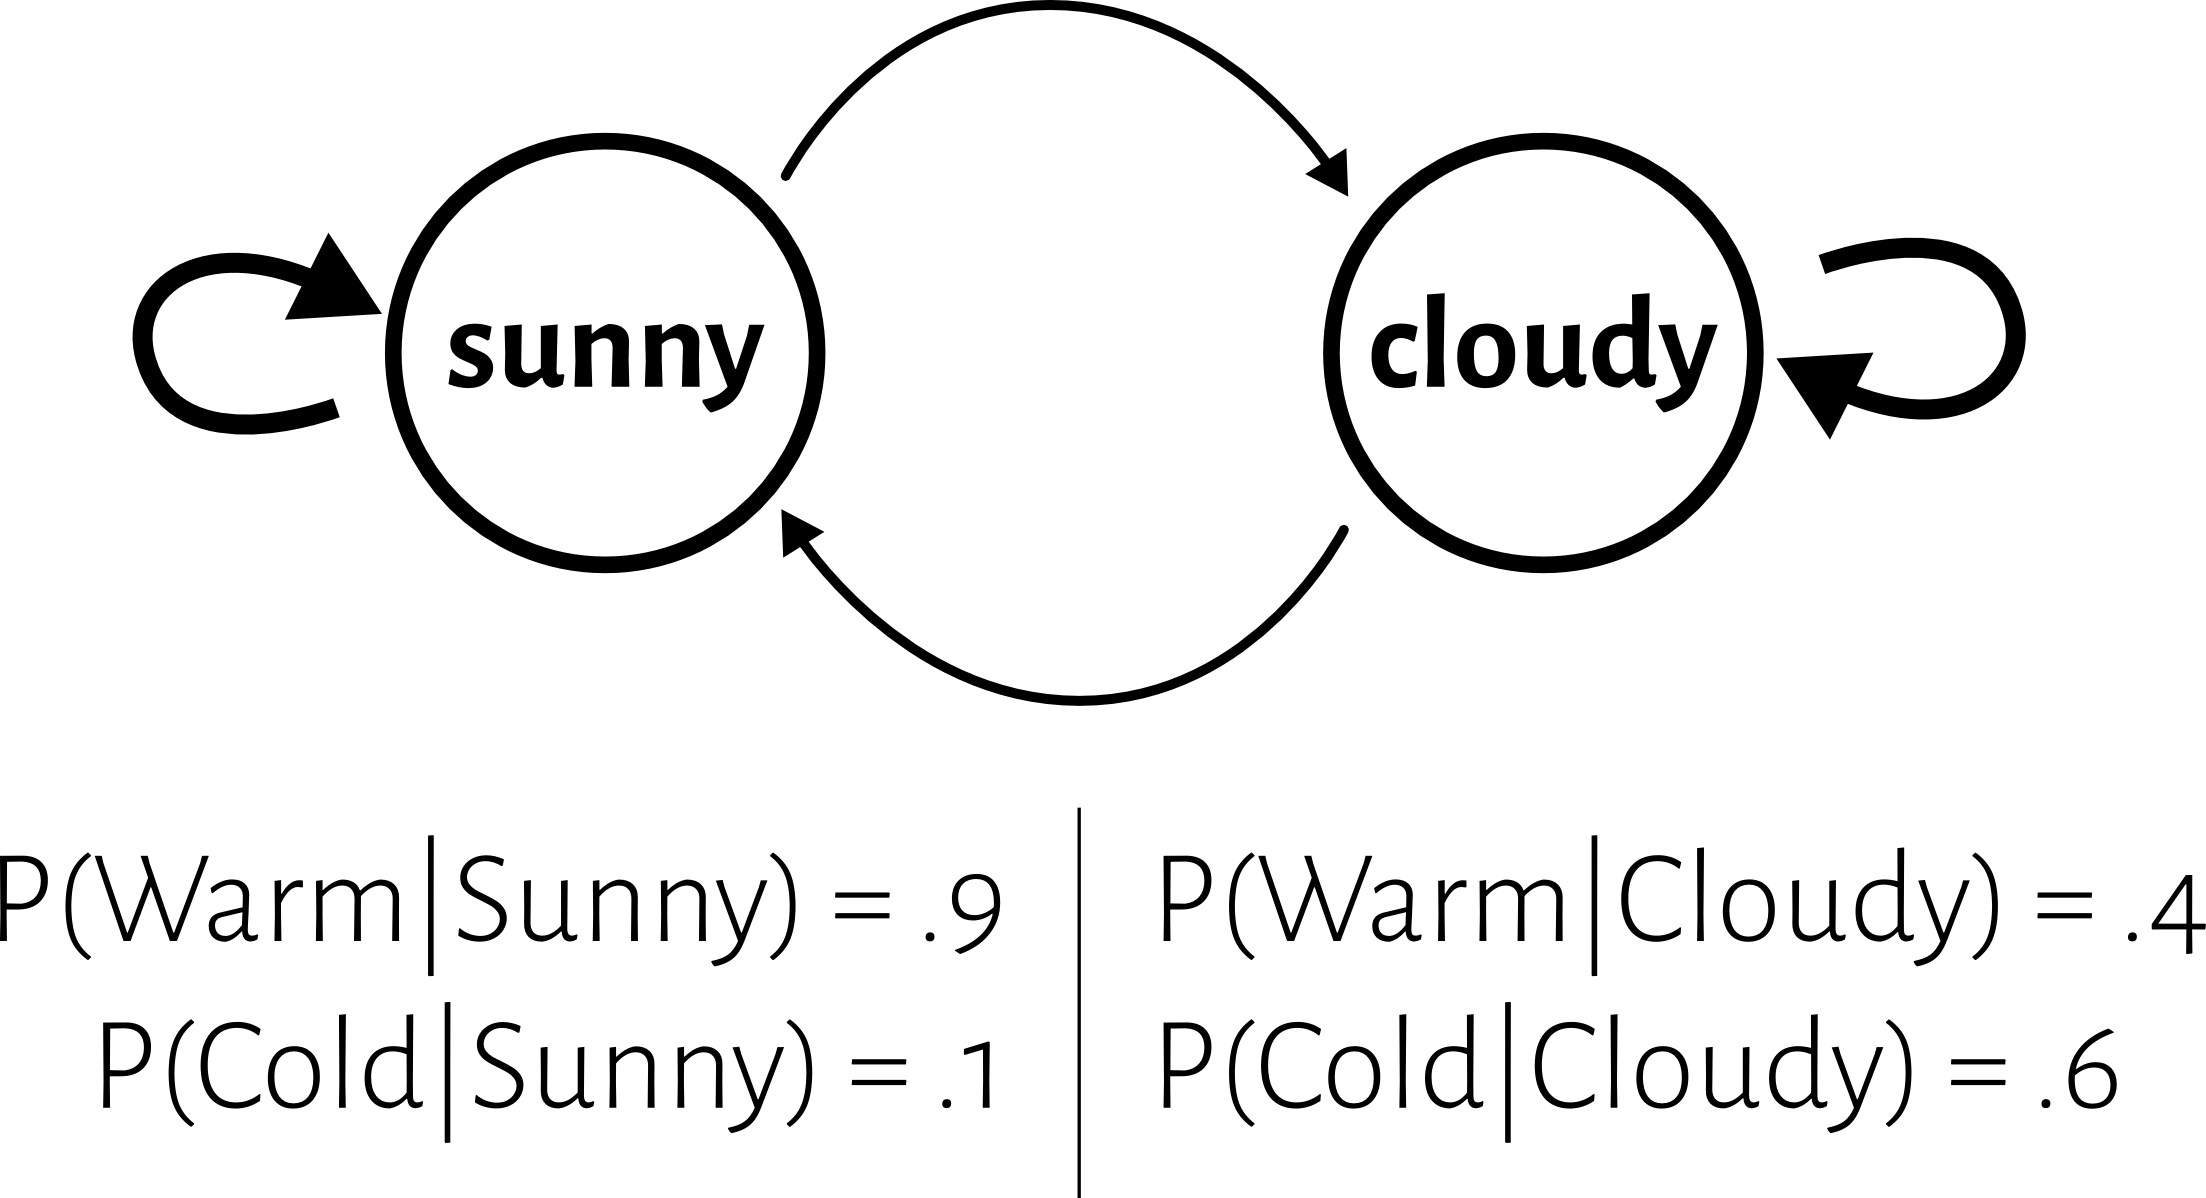
\includegraphics[width=0.5\textwidth]{../figures/g5016.png}
%\caption{A 2-state Markov chain}
%\end{figure}

In contrast, a \textbf{hidden Markov model} is a Markov process with unobserved or ``hidden'' states. However, we do have some noisy information about the states as each state emits observations according to a probability distribution that is characteristic of that state. We see the resulting emissions generated from the process and are not sure of the true underlying state of the Markov process at each given time point. Inferring information about the states of these processes and the probabilities that govern how such processes work has a wide range of applications, particularly for studying sequential data in which we are fairly certain the Markov property is satisfied.

In graphical model notation, an HMM is often represented as in Figure~\ref{fig:pgm}. This clearly shows that the HMM is a series of states with an observation (or emission) generated by each state. Only the emissions are observed and this is depicted by the shading of the respective nodes.

\begin{figure}[H]
\centering
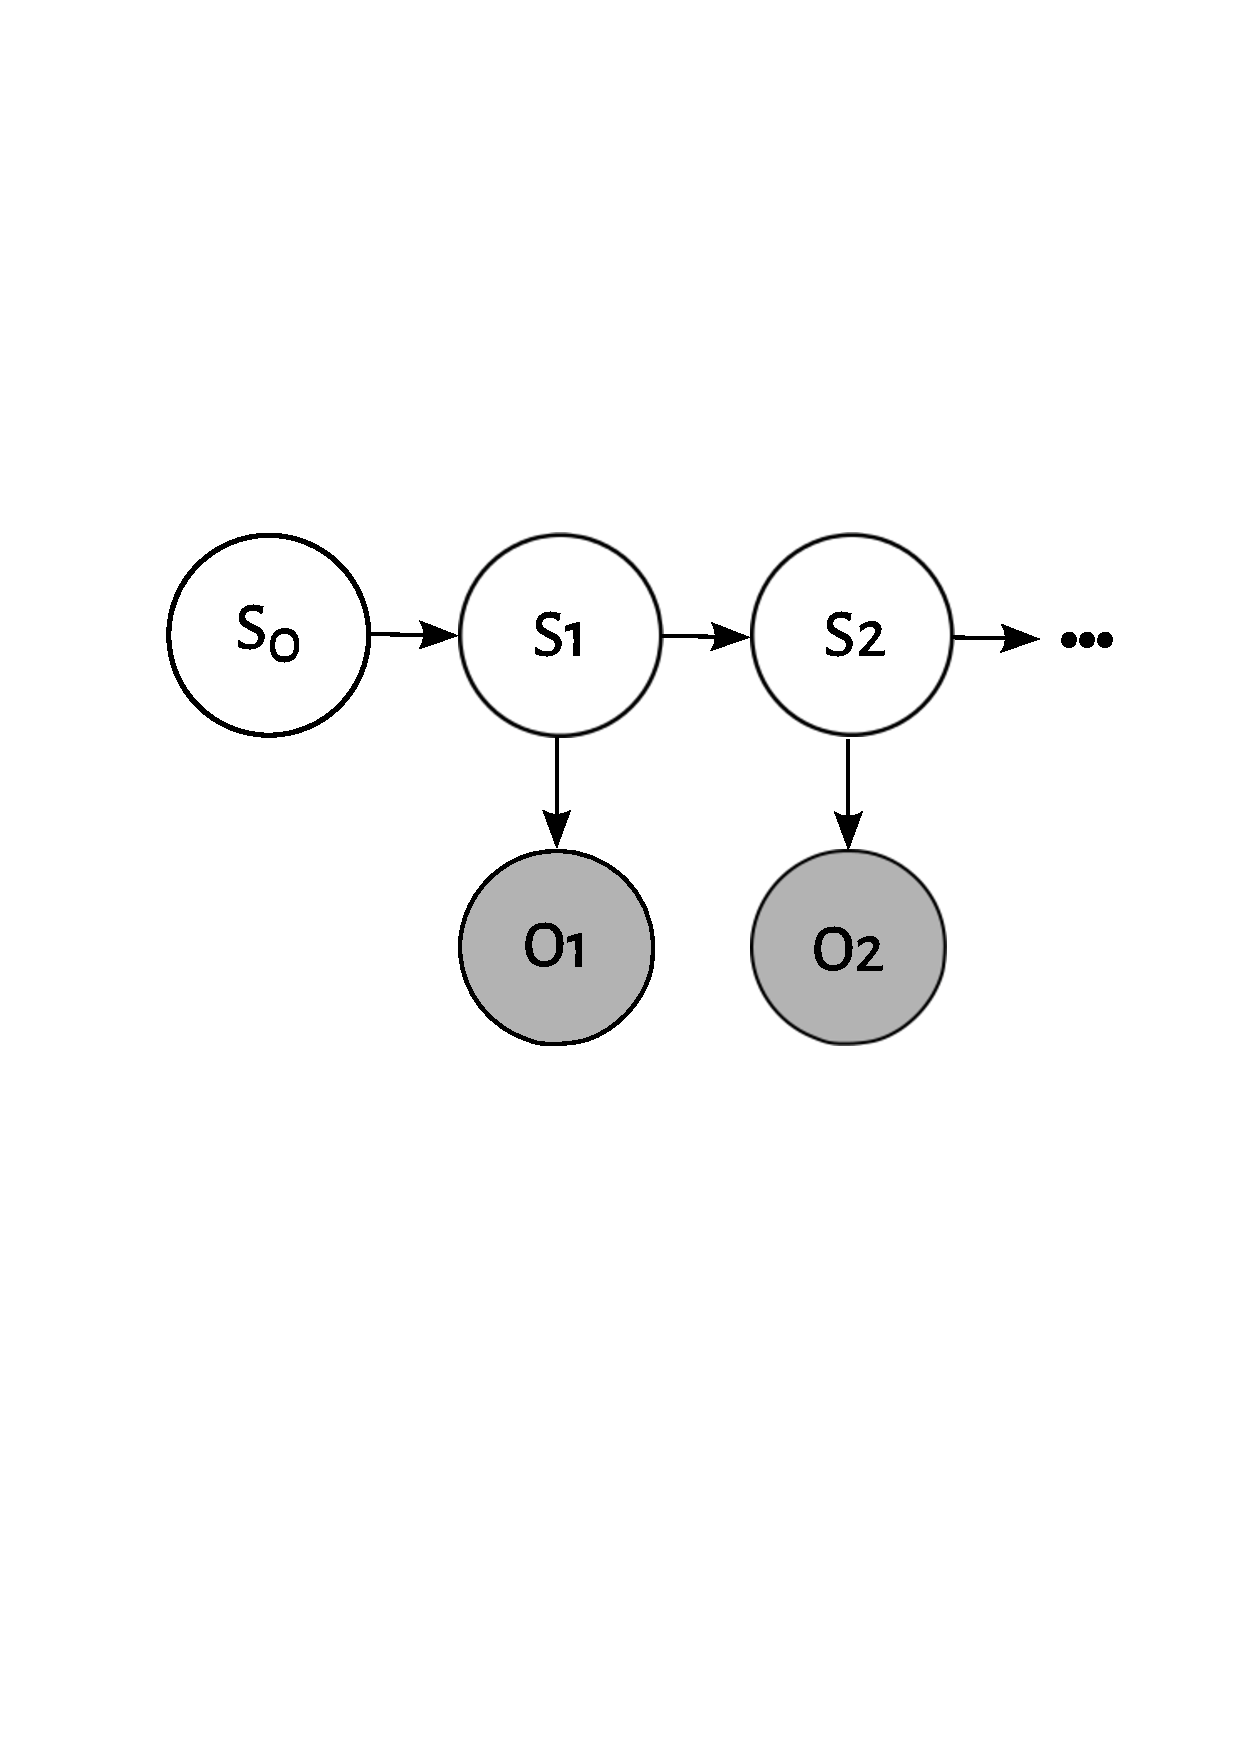
\includegraphics[width=0.5\textwidth]{../figures/hmmTemplate.pdf}
\caption{General graphical model depiction of an HMM}
\label{fig:pgm}
\end{figure}

\subsection{What kind of data is well modeled by a HMM?}
Sequential data are really well modeled by HMMs, especially when we are interested in assigning a label to a specific segment of the sequence. Examples of these kinds of data are time series data and DNA sequence data - the latter of which concerns us most. 

\subsection{Well-known examples of HMMs in biology}

\begin{itemize}
\item Gene finding (GENSCAN: \url{http://www.ncbi.nlm.nih.gov/pubmed/9149143}, \url{http://genes.mit.edu/GENSCAN.html})
\item Modeling protein sequences and homologs (HMMER: \url{http://hmmer.janelia.org/})
\item Chromatin state annotation (ChromHMM: \url{http://www.ncbi.nlm.nih.gov/pubmed/22373907}, \url{http://compbio.mit.edu/ChromHMM/})
\end{itemize}

\section{Algorithms}
\subsection{Formal Definition of a HMM}
An HMM is defined by:
\begin{itemize}
\item A set of $s$ states.
\item An alphabet of $n$ possible emissions from each state.
\item A vector of length $s$ where the $i$th entry is the probability of starting in state $i$.
\item An $s\times s$ transition matrix $A$ where $A_{ij}$ is the probability of going from state $i$ to state $j$.
\item An $s \times n$ emission matrix $B$ where $B_{ij}$ is the probability that state $i$ emits symbol $j$.
\end{itemize}

\subsection{Assumptions}
The state at time $t$ depends only on the state at time $t-1$.\\
The transition and emission probabilities are constant over time.
\subsection{Interpretation}
\subsection{The Viterbi Algorithm}
\subsection{The Baum-Welch Algorithm}

This is the algorithm used to learn the parameters of an HMM given unlabeled training data. 
It is a special case of the expectation-maximization (EM) algorithm. These types of algorithms work by iterating over two steps: the E-step and the M-step.

In the case of HMMs, if we knew the state that each emission came from, then we could easily infer the emission and transition probabilities (we will do this in Exercise 1). However, in the case of unlabeled data, we do not have this information. The idea is therefore to initialize the parameters with some values then find the most likely state assignment (E-step). With that assignment in hand, we now have labeled data and can use maximum likelihood estimation to update our estimates for the emission and transition parameter values (M-step). We keep iterating between the E- and M-steps until convergence. It is important to note that we may not arrive at an optimal solution. Different initializations of the parameter values can lead to different results.

The inference of the most likely sequence of states (E-Step) is done with the forward-backward algorithm. The forward-backward algorithm returns a probability distribution over the states for each emission. If you want to use hard EM, you would select the single most likely state (i.e. the state with the highest assigned probability). A better idea is to use soft EM where you keep the soft assignments to states (i.e. the probability distribution).

\subsection{Caveats}

\section{Exercise 1}
Consider a simple two-state HMM that models the GC content of a DNA sequence. 
There is a state to represent GC-rich regions and another for regions that are not GC rich.
You have a sequence of observed emissions. 
And you also happen to know which state generated each emission (lucky you!). 
Given these data, you will estimate the parameters of the HMM. 

[Use starter code in exercise1.R]

\subsection{Estimate the emission probabilities for each of the two states}
\begin{table}[H]
\centering
\begin{tabular}{|c|c|c|c|c|}
\hline
& A & T & G & C \\\hline
GC rich & & & &  \\\hline
not GC rich & & & & \\\hline
\end{tabular}
\end{table}

\subsection{Estimate the transition probabilities between states}
\begin{table}[H]
\centering
\begin{tabular}{|c|c|c|}
\hline
& GC rich & not GC rich \\\hline
GC rich & &  \\\hline
not GC rich & &  \\\hline
\end{tabular}
\end{table}

\section{Exercise 2}
Consider an HMM of the same form as before. 
Again you observe a sequence of emissions. 
However, this time the states are also unknown. 
This time we will learn the parameters of the HMM without knowing the true sequence of states that generated the observations! 

[Use starter code in exercise2.R]

\subsection{Estimate the parameters of the HMM}
Emission probabilities
\begin{table}[H]
\centering
\begin{tabular}{|c|c|c|c|c|}
\hline
& A & T & G & C \\\hline
GC rich & & & &  \\\hline
not GC rich & & & & \\\hline
\end{tabular}
\end{table}

Transition probabilities
\begin{table}[H]
\centering
\begin{tabular}{|c|c|c|}
\hline
& GC rich & not GC rich \\\hline
GC rich & &  \\\hline
not GC rich & &  \\\hline
\end{tabular}
\end{table}

\subsection{Predict the most likely state sequence using the parameters you just estimated}

\end{document} 
